\documentclass{beamer}
\usetheme{Boadilla}

\usepackage{amsmath}
\usepackage{IEEEtrantools}
\usepackage{subfig}
\usepackage{color}
\usepackage{bibentry}
\nobibliography*

% General things
\newcommand{\half}{\frac{1}{2}}
\newcommand{\pdv}[2]{\frac{\partial #1}{\partial #2}}
\newcommand{\pd}[3]{\left.\frac{\partial #1}{\partial #2}\right|_{#3}}
\newcommand{\determ}[1]{\left| #1 \right|}

% Density families
\newcommand{\normalden}[3]{\mathcal{N}\left(#1\left|#2,#3\right.\right)}       % Normal density

% Basics
\newcommand{\ti}{n}                             % Time index
\newcommand{\pt}{\lambda}                       % Pseudo-time
\newcommand{\ls}[1]{x_{#1}}                     % Latent state
\newcommand{\ob}[1]{y_{#1}}                     % Observation
\newcommand{\stdnorm}[1]{z_{#1}}                % Standard normal R.V.

% Densities
\newcommand{\den}{p}                            % Secondary Bayesian density
\newcommand{\transden}{f}                       % Transition density
\newcommand{\obsden}{g}                         % Observation density
\newcommand{\impden}{q}                         % Importance density
\newcommand{\partden}{\eta}                     % Unweighted particle distribution
\newcommand{\artden}{\rho}                      % Artificial conditional density
\newcommand{\oiden}[1]{\pi_{#1}}                % Optimal importance density
\newcommand{\augfiltden}[1]{\tilde{\pi}_{#1}}   % Augmented filtering density


% Particle shizzle
\newcommand{\pss}[2][]{^{(#2)#1}}               % Particle superscript
\newcommand{\pw}[1]{w_{#1}}                     % Particle weight

% Models
\newcommand{\transfun}{\phi}                    % Transition function
\newcommand{\obsfun}{\psi}                      % Observation function
\newcommand{\transcov}{Q}                       % Transition covariance
\newcommand{\obscov}{R}                         % Observation covariance
\newcommand{\obsmat}{H}                         % Linear observation matrix 
\newcommand{\obsmatapprox}[1]{\hat{\obsmat}_{#1}} % Linear observation matrix formed by differentiation of the observation function

% Gaussian moments
\newcommand{\lsmn}[1]{m_{#1}}                   % Mean
\newcommand{\lsvr}[1]{P_{#1}}                   % Variance
\newcommand{\obmn}[1]{\mu_{#1}}
\newcommand{\obvr}[1]{\Sigma_{#1}}
\newcommand{\obcvr}[1]{C_{#1}}

% Simulation models - tracking
\newcommand{\pos}[1]{p_{#1}}                    % Position
\newcommand{\vel}[1]{v_{#1}}                    % Velocity
\newcommand{\bng}[1]{\theta_{#1}}               % Bearing
\newcommand{\rng}[1]{r_{#1}}                    % Range
\newcommand{\hei}[1]{h_{#1}}                    % Height
\newcommand{\rngrt}[1]{s_{#1}}                  % Range rate
\newcommand{\terrain}{T}                        % Terrain height
\graphicspath{{../../paper/figures/}{CAMSAP_plots/}}
\captionsetup[subfloat]{labelformat=empty}

\title[Progressive Proposals]{Particle Filtering with Progressive Gaussian Approximations to the Optimal Importance Density}
\author[P. Bunch \& S. Godsill]{Pete Bunch and Simon Godsill}
\institute[CUED SigProC]{Cambridge University Engineering Department\\ Signal Processing \& Communications Lab}
\date{17th December, 2012}

\begin{document}

\begin{frame}
 \titlepage
\end{frame}
\begin{frame}{The Plan}
 \begin{itemize}
  \item A quick review of particle filtering and importance densities.
  \item The problem with the usual choices of importance density.
  \item The new progressive proposal method.
  \item How it relates to existing algorithms.
  \item Some simulation results.
 \end{itemize}
\end{frame}


\begin{frame}{Particle Filtering}
\begin{IEEEeqnarray*}{rCcCl}
 \ls{\ti} & \sim & \transden(\ls{\ti} | \ls{\ti-1}) & = & \normalden{\ls{\ti}}{\transfun(\ls{\ti-1})}{\transcov} \\
 \ob{\ti} & \sim & \obsden(\ob{\ti} | \ls{\ti})     & = & \normalden{\ob{\ti}}{\obsfun(\ls{\ti})}{\obscov} \\
 \ls{1} & \sim & p(\ls{1})                          & = & \normalden{\ls{1}}{\lsmn{1}}{\lsvr{1}}      ,
\end{IEEEeqnarray*}
\pause
\begin{itemize}
 \item Particle filter approximates:
 \begin{IEEEeqnarray*}{rCl}
  \den(\ls{1:\ti}|\ob{1:\ti}) & \propto & \transden(\ls{\ti}|\ls{\ti-1}) \obsden(\ob{\ti}|\ls{\ti}) \den(\ls{1:\ti-1}|\ob{1:\ti-1})
 \end{IEEEeqnarray*}
 \item Select an ($\ti-1$) particle and sample a new state, $\ls{\ti}\pss{i} \sim \impden(\ls{\ti}|\ls{\ti-1}\pss{i})$.
 \item Update weight $\pw{\ti}\pss{i} = \frac{ \transden(\ls{\ti}\pss{i}|\ls{\ti-1}\pss{i}) \obsden(\ob{\ti}|\ls{\ti}\pss{i}) }{ \impden(\ls{\ti}\pss{i}|\ls{\ti-1}\pss{i}) }$.
\end{itemize}
\end{frame}
\begin{frame}{Importance Densities}
\pause Bootstrap filter
\begin{IEEEeqnarray*}{rCl}
 \impden(\ls{\ti}|\ls{\ti-1}) = \transden(\ls{\ti}|\ls{\ti-1})     .
\end{IEEEeqnarray*}
\pause Optimal Importance Density
\begin{IEEEeqnarray*}{rCl}
 \impden(\ls{\ti}|\ls{\ti-1}) = \frac{ \transden(\ls{\ti}|\ls{\ti-1}) \obsden(\ob{\ti}|\ls{\ti}) }{ \int \transden(\ls{\ti}|\ls{\ti-1}) \obsden(\ob{\ti}|\ls{\ti}) d\ls{\ti} }      .
\end{IEEEeqnarray*}
Approximate by linearisation or sigma-point approximation.
\end{frame}


\begin{frame}{An Example}
\begin{figure}
\centering
\subfloat[Prior]{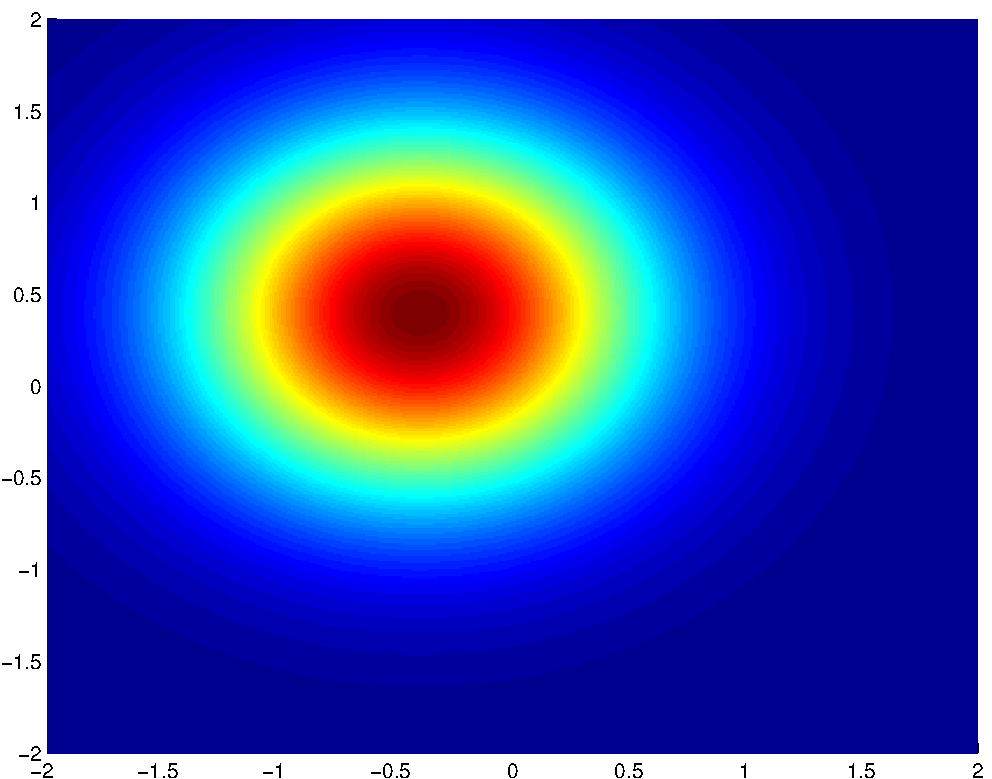
\includegraphics[width=0.5\columnwidth]{path_ex_prior.pdf}}
\subfloat[Likelihood]{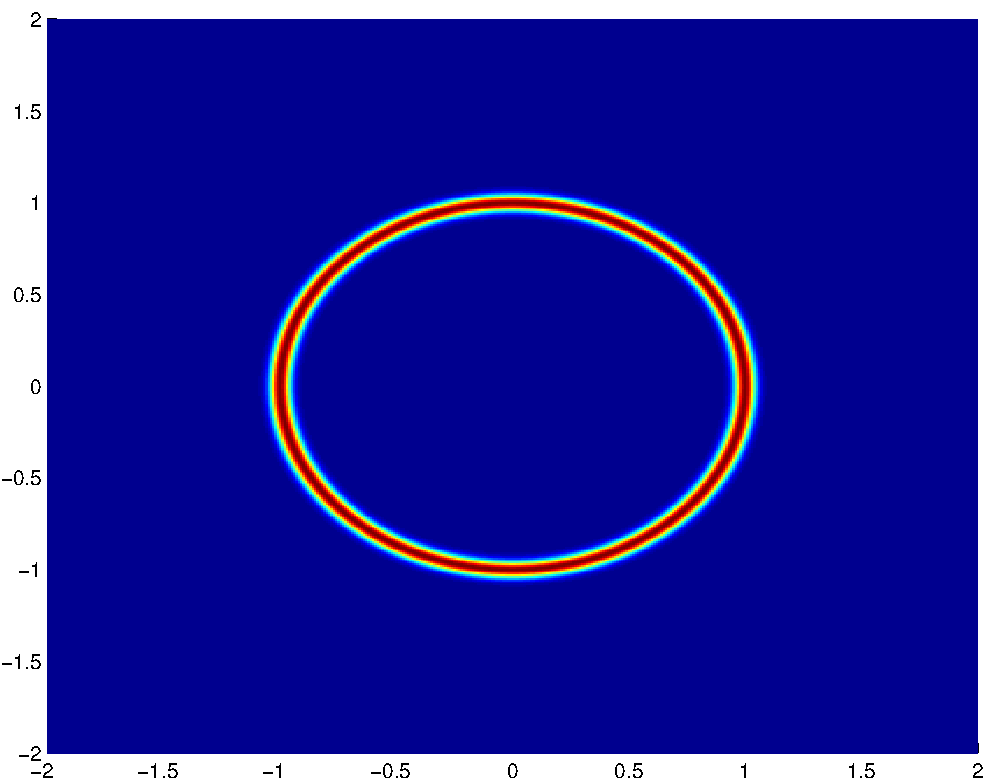
\includegraphics[width=0.5\columnwidth]{path_ex_lhood.pdf}}
\end{figure}
\end{frame}
\begin{frame}{An Example - Linearisation}
\begin{figure}
\centering
\subfloat[True Posterior]{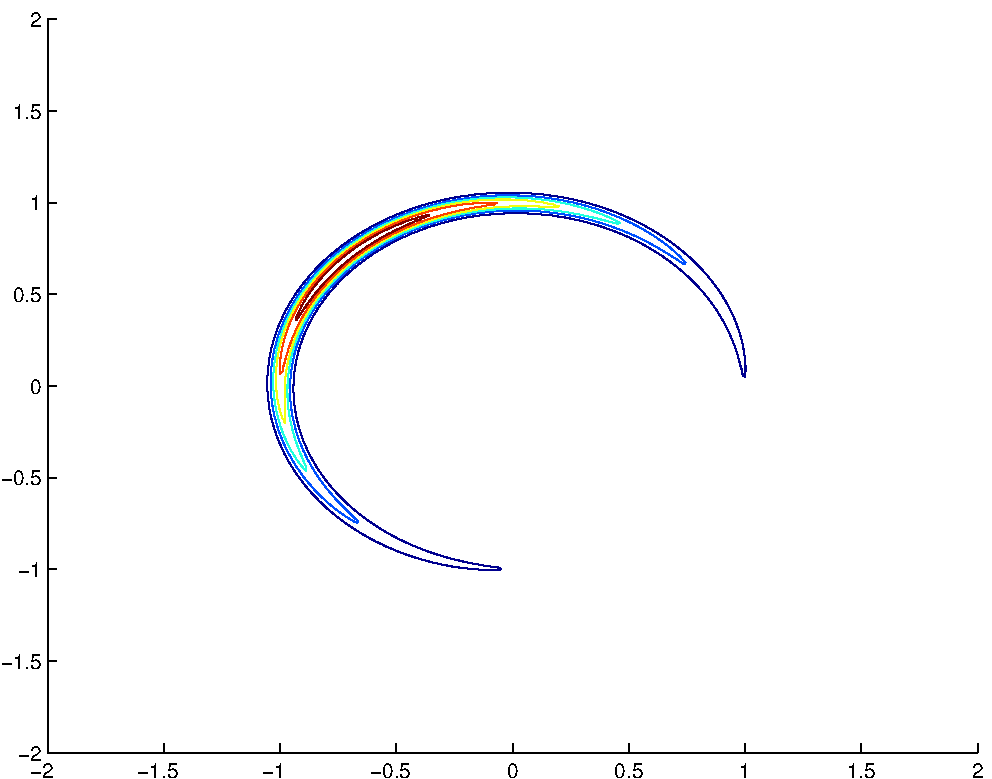
\includegraphics[width=0.5\columnwidth]{path_ex_post_contour.pdf}}
\subfloat[Approximated by Linearisation]{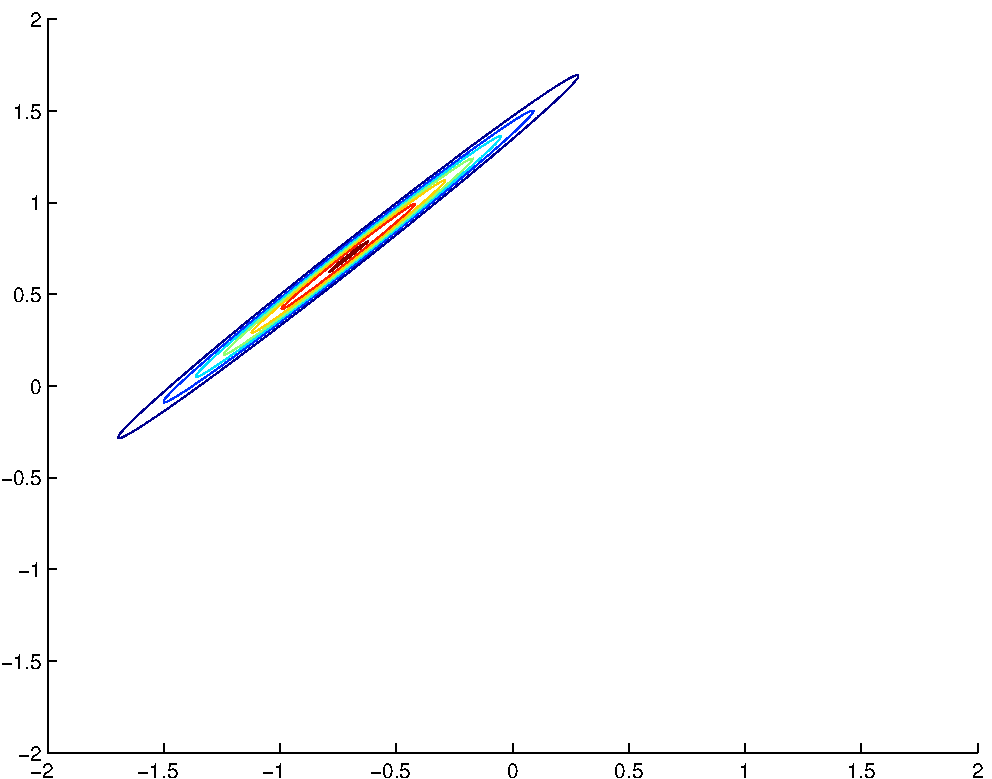
\includegraphics[width=0.5\columnwidth]{path_ex_ekf.pdf}}
\end{figure}
\end{frame}
\begin{frame}{An Example - Unscented Transform}
\begin{figure}
\centering
\subfloat[True Posterior]{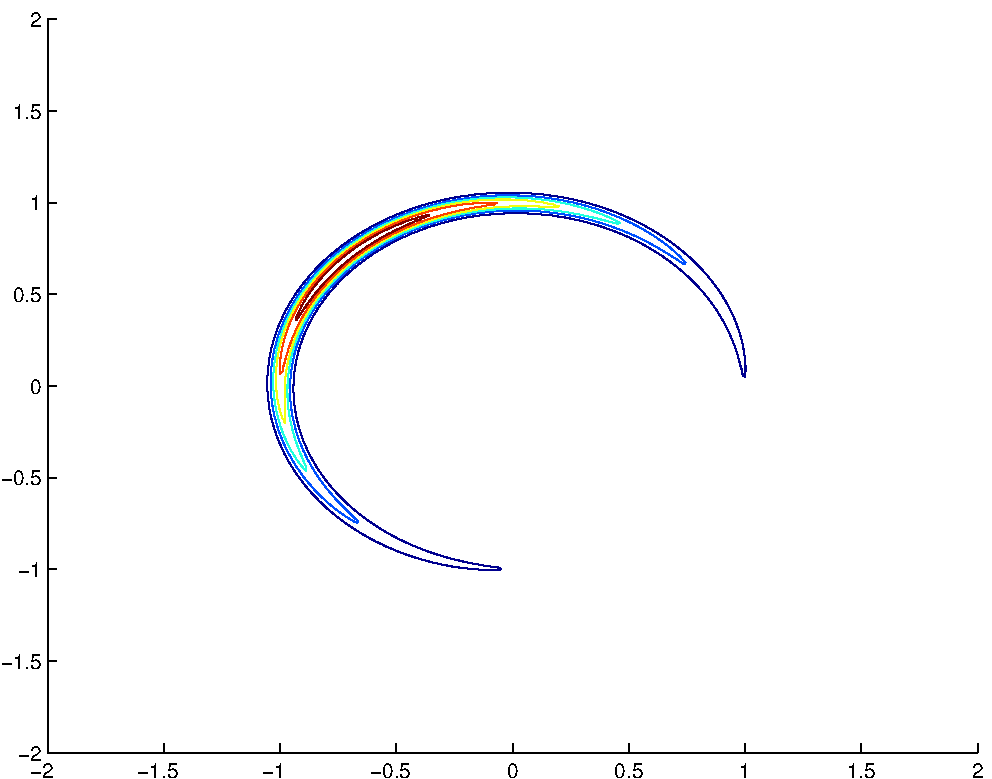
\includegraphics[width=0.5\columnwidth]{path_ex_post_contour.pdf}}
\subfloat[Approximated by Unscented Transform]{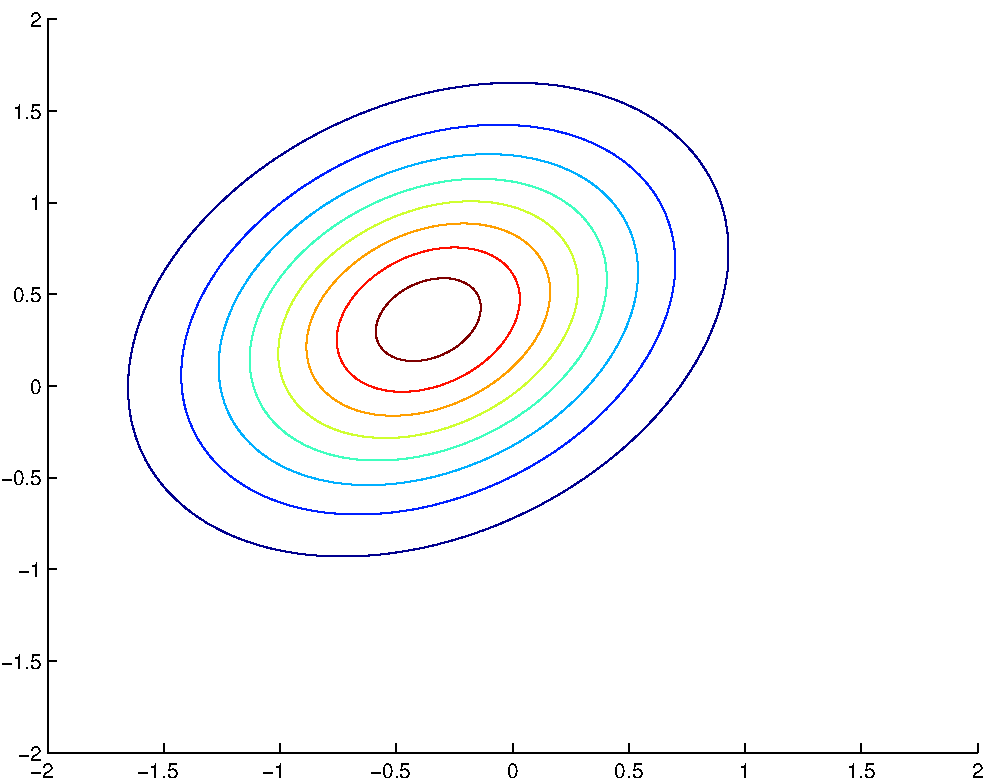
\includegraphics[width=0.5\columnwidth]{path_ex_ukf.pdf}}
\end{figure}
\end{frame}


\begin{frame}{Progressive Principle}
Introduce the observation gradually using a stretch of ``pseudo-time'', $\pt \in [0,1]$. \\
\vspace{1em}
\pause
Smooth sequence of target distributions:
 \begin{IEEEeqnarray*}{rCl}
 \augfiltden{\ti,\pt}(\ls{1:\ti-1}, \ls{\ti,\pt}) & \propto & \obsden(\ob{\ti} | \ls{\ti,\pt})^{\pt} \transden(\ls{\ti,\pt} | \ls{\ti-1}) p(\ls{1:\ti-1}|\ob{1:\ti-1})
\end{IEEEeqnarray*}
\pause
Smooth sequence of optimal importance densities:
\begin{IEEEeqnarray*}{rCl}
 \oiden{\ti,\pt}(\ls{\ti,\pt} | \ls{\ti-1}\pss{j}) & \propto & \obsden(\ob{\ti} | \ls{\ti,\pt})^{\pt} \transden(\ls{\ti,\pt} | \ls{\ti-1}\pss{j})
\end{IEEEeqnarray*}
\end{frame}
\begin{frame}{Partially Linear Gaussian Models}
\begin{IEEEeqnarray*}{rCl}
 \transden(\ls{\ti}|\ls{\ti-1}) & = & \normalden{\ls{\ti}}{\transfun(\ls{\ti-1})}{\transcov} \\
 \obsden(\ob{\ti}|\ls{\ti})     & = & \normalden{\ob{\ti}}{\obsmat \ls{\ti}}{\obscov}
\end{IEEEeqnarray*}
\vspace{1em}
\pause
Optimal importance density is analytically tractable.
\begin{IEEEeqnarray*}{rCl}
 \oiden{\pt}(\ls{\pt} | \ls{\ti-1}) & = & \normalden{\ls{\pt}}{\lsmn{\pt}}{\lsvr{\pt}}    ,
\end{IEEEeqnarray*}
\begin{IEEEeqnarray*}{rCl}
 \lsvr{\pt}  & = & \left[ \transcov^{-1} + \pt \obsmat^T \obscov^{-1} \obsmat \right]^{-1} \\
 \lsmn{\pt} & = & \lsvr{\pt} \left[ \transcov^{-1} \transfun(\ls{\ti-1}) + \pt \obsmat^T \obscov^{-1} \ob{\ti} \right]       .
\end{IEEEeqnarray*}
\end{frame}
\begin{frame}{Partially Linear Gaussian Models}
Any Gaussian random variable may be expressed as,
\begin{IEEEeqnarray*}{rCl}
 \ls{} & = & \lsmn{} + \lsvr{}^{\half} \stdnorm{} \\
 \stdnorm{} & \sim & \normalden{\stdnorm{}}{0}{I}      .
\end{IEEEeqnarray*}
\pause
Progress particle from $\pt_0$ to $\pt_1$ with a linear transformation.
\begin{IEEEeqnarray*}{rCl}
 \ls{\pt_1} & = & \lsmn{\pt_1} + \lsvr{\pt_1}^{\half}\lsvr{\pt_0}^{-\half}(\ls{\pt_0}-\lsmn{\pt_0})       .
\end{IEEEeqnarray*}
If $\ls{\pt_0} \sim \oiden{\pt_0}(\ls{\pt_0}|\ls{\ti-1})$, then $\ls{\pt_1} \sim \oiden{\pt_1}(\ls{\pt_1}|\ls{\ti-1})$
\end{frame}
\begin{frame}{Partially Linear Gaussian Models}
\begin{figure}
\centering
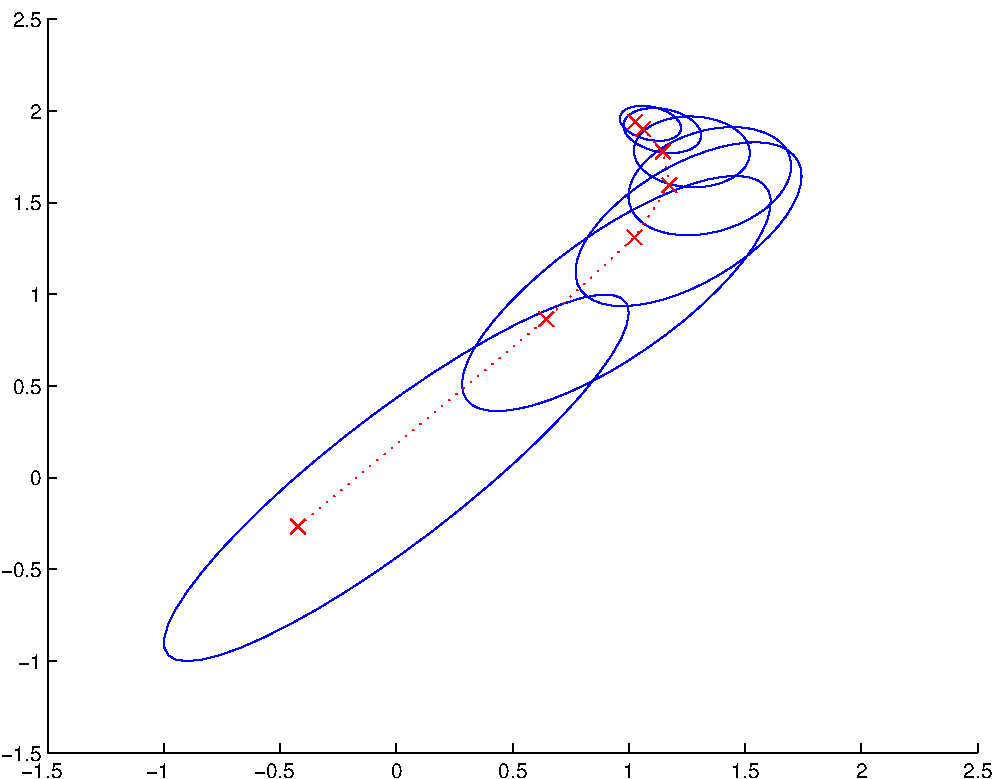
\includegraphics[width=0.5\columnwidth]{plg_oid_evolution.pdf}
\end{figure}
\end{frame}

\begin{frame}{Nonlinear Gaussian Models}
\begin{IEEEeqnarray*}{rCl}
 \transden(\ls{\ti} | \ls{\ti-1}) & = & \normalden{\ls{\ti}}{\transfun(\ls{\ti-1})}{\transcov} \\
 \obsden(\ob{\ti} | \ls{\ti})     & = & \normalden{\ob{\ti}}{\obsfun(\ls{\ti})}{\obscov}
\end{IEEEeqnarray*}
\pause
Approximate the optimal importance density with a Gaussian at each point in pseudo-time.
\begin{IEEEeqnarray*}{rCl}
 \oiden{\pt}(\ls{\pt} | \ls{\ti-1}) & \approx & \normalden{\ls{\pt}}{\lsmn{\pt}}{\lsvr{\pt}}
\end{IEEEeqnarray*}
\vspace{1em}
\pause
To update from $\pt_0$ to $\pt_1$,
\begin{IEEEeqnarray*}{rCl}
 \oiden{\pt_1}(\ls{}|\ls{\ti-1}) & \propto & \oiden{\pt_0}(\ls{}|\ls{\ti-1}) \obsden(\ob{\ti}|\ls{})^{\pt_1-\pt_0} \\
 & \propto & \normalden{\ls{}}{\lsmn{\pt_0}}{\lsvr{\pt_0}} \normalden{\ob{\ti}}{\obsfun(\ls{})}{\obscov}^{\pt_1-\pt_0} \\
 & \propto & \normalden{\ls{}}{\lsmn{\pt_0}}{\lsvr{\pt_0}} \normalden{\ob{\ti}}{\obsfun(\ls{})}{\frac{\obscov}{\pt_1-\pt_0}}      .
\end{IEEEeqnarray*}
\end{frame}
\begin{frame}{Nonlinear Gaussian Models}
Approximate with linearisation.
\begin{IEEEeqnarray*}{rCl}
 \obsmatapprox{\ls{\pt_0}} & = & \pd{\obsfun}{\ls{}}{\ls{\pt_0}}
\end{IEEEeqnarray*}
\pause
\vspace{1em}
\begin{IEEEeqnarray*}{rCl}
 \obmn{\pt_0}  & = & \obsfun(\ls{\pt_0}) + \obsmatapprox{\ls{\pt_0}} ( \lsmn{\pt_0} - \ls{\pt_0} ) \nonumber \\
 \obvr{\pt_0}  & = & \obsmatapprox{\ls{\pt_0}} \lsvr{\pt_0} \obsmatapprox{\ls{\pt_0}}^T \\
 \obcvr{\pt_0} & = & \lsvr{\pt_0} \obsmatapprox{\ls{\pt_0}}^T \\
 \lsmn{\pt_1}  & = & \lsmn{\pt_0} + \obcvr{\pt_0} \left(\obvr{\pt_0}+ \frac{\obscov}{\pt_1-\pt_0}\right)^{-1} \left(\ob{\ti}-\obmn{\pt_0}\right)  \\
 \lsvr{\pt_1}  & = & \lsvr{\pt_0} - \obcvr{\pt_0} \left(\obvr{\pt_0}+ \frac{\obscov}{\pt_1-\pt_0}\right)^{-1} \obcvr{\pt_0}^T
\end{IEEEeqnarray*}
\end{frame}

\begin{frame}{Weight Evolution}
\begin{itemize}
 \item Existing particle at pseudo time $\pt_0$,
 \begin{IEEEeqnarray*}{rCl}
  \left\{ \ls{1:\ti-1}\pss{i}, \ls{\pt_0}\pss{i} \right\} \sim \partden_{\pt_0}(\ls{1:\ti-1}, \ls{\pt_0})     .
 \end{IEEEeqnarray*}
 \item ... is replaced by new particle  at $\pt_1$,
 \begin{IEEEeqnarray*}{rCl}
  \left\{ \ls{1:\ti-1}\pss{i}, \ls{\pt_1}\pss{i} \right\} \sim \partden_{\pt_1}(\ls{1:\ti-1}, \ls{\pt_1})     .
 \end{IEEEeqnarray*}
\pause
 \item Standard change of variables formula,
 \begin{IEEEeqnarray*}{rCl}
  \partden_{\pt_1}(\ls{1:\ti-1},\ls{\pt_1}) & = & \partden_{\pt_0}(\ls{1:\ti-1},\ls{\pt_0}) \times \determ{ \pdv{\ls{\pt_0}}{\ls{\pt_1}} } \nonumber      .
 \end{IEEEeqnarray*}
\end{itemize}
\end{frame}
\begin{frame}{Weight Evolution}
Hence weight update,
\begin{IEEEeqnarray*}{rCl}
 \pw{\pt_1} & = & \frac{ \augfiltden{\pt_1}(\ls{1:\ti-1},\ls{\pt_1}) }{ \partden_{\pt_1}(\ls{1:\ti-1},\ls{\pt_1}) } \nonumber \\
 & = & \frac{ \augfiltden{\pt_0}(\ls{1:\ti-1},\ls{\pt_0}) }{ \partden_{\pt_0}(\ls{1:\ti-1},\ls{\pt_0}) } \times \frac{ \augfiltden{\pt_1}(\ls{1:\ti-1},\ls{\pt_1})}{ \augfiltden{\pt_0}(\ls{1:\ti-1},\ls{\pt_0}) } \times \determ{ \pdv{\ls{\pt_1}}{\ls{\pt_0}} } \nonumber \\
 & \propto & \pw{\pt_0} \times \frac{ \obsden(\ob{\ti} | \ls{\pt_1})^{\pt_1} \transden(\ls{\pt_1} | \ls{\ti-1}) }{ \obsden(\ob{\ti} | \ls{\pt_0})^{\pt_0} \transden(\ls{\pt_0} | \ls{\ti-1}) } \times \sqrt{\frac{\determ{\lsvr{\pt_1}}}{\determ{\lsvr{\pt_0}}}}      .
\end{IEEEeqnarray*}
\end{frame}

\begin{frame}{Relationship to Other Methods}
Gradual introduction of likelihood underlies numerous existing particle methods,
{\tiny
\begin{itemize}
 \item \bibentry{Godsill2001b}
 \item \bibentry{Gall2007}
 \item \bibentry{Deutscher2000}
 \item \bibentry{Oudjane2000}
 \item \bibentry{Daum2008}
 \item \bibentry{Reich2011}
\end{itemize}
}
\end{frame}
\begin{frame}{Relationship to Other Methods}
Distinguishing features of the new progressive proposal method:
\begin{itemize}
 \item Particles moved deterministically.
 \item Move one particle at a time --- no intermediate interaction steps needed.
 \item Adaptive step-size control for \emph{each particle}.
\end{itemize}
\end{frame}


\begin{frame}{Simulations - A Tracking Problem}
\begin{IEEEeqnarray*}{rCl}
 \ls{\ti} & = & \begin{bmatrix} \pos{\ti}^T & \vel{\ti}^T \end{bmatrix}^T
\end{IEEEeqnarray*}
Near-constant velocity model.
\pause
\begin{IEEEeqnarray*}{rCl}
 \ob{\ti} & = & \begin{bmatrix} \bng{\ti} & \rng{\ti} & \hei{\ti} & \rngrt{\ti} \end{bmatrix}^T       .
\end{IEEEeqnarray*}
\begin{IEEEeqnarray*}{rCl}
 \bng{\ti}   & = & \arctan\left(\frac{\pos{\ti,1}}{\pos{\ti,2}}\right)\\
 \rng{\ti}   & = & \sqrt{ \pos{\ti,1}^2 + \pos{\ti,3}^2 + \pos{\ti,3}^2 } \\
 \hei{\ti}   & = & \pos{\ti,3} - \terrain( \pos{\ti,1}, \pos{\ti,2} ) \\
 \rngrt{\ti} & = & \frac{ \pos{\ti}\cdot\vel{\ti} }{ \rng{\ti} }       ,
\end{IEEEeqnarray*}
\end{frame}
\begin{frame}{Simulations - Terrain Map}
\begin{IEEEeqnarray*}{rCl}
 \terrain( \pos{\ti,1}, \pos{\ti,2} )
\end{IEEEeqnarray*}
\begin{figure}
\centering
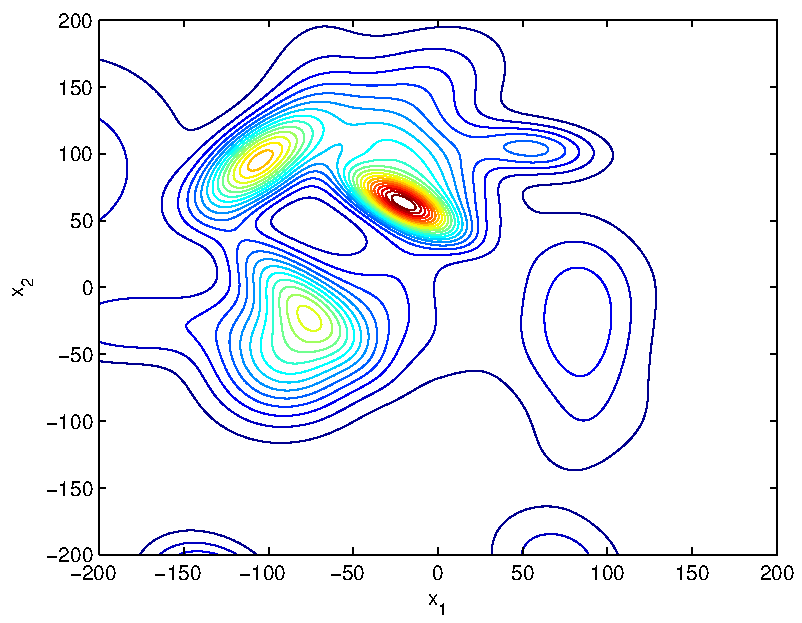
\includegraphics[width=0.5\columnwidth]{drone_terrain_map.pdf}
\end{figure}
\end{frame}
\begin{frame}{Simulations - Results}
\begin{figure}
\centering
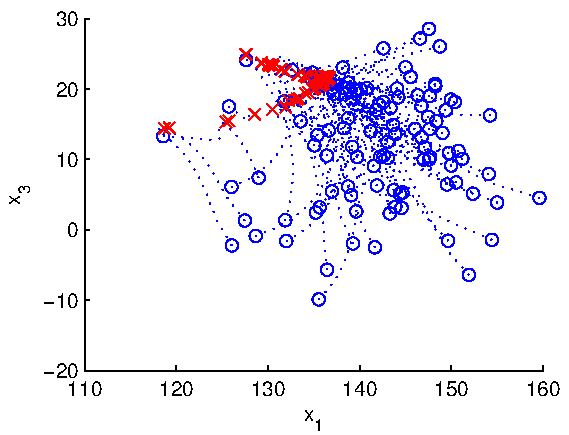
\includegraphics[width=0.5\columnwidth]{drone_example_frame_deter.pdf}
\end{figure}
\end{frame}
\begin{frame}{Simulations - Results}
\begin{table}
\centering
\begin{tabular}{l||c|c|c}
Algorithm                                & $N_F$ & ESS  & RMSE \\
\hline
Bootstrap Proposal                       &  6000 &  1.0 & 78.6 \\
Unscented Kalman Proposal                &   460 &  2.4 & 70.2 \\
Gaussian Local Maximum Proposal          &    10 &  3.1 & 62.9 \\
Progressive Proposal                     &   180 & 56.4 & 22.3 \\
\end{tabular}
\end{table}
\end{frame}

\begin{frame}{Summary}
\begin{itemize}
 \item The progressive proposal method samples from an effective approximation of the optimal importance density.
 \item Particles sampled from the transition density, then moved deterministically with a series of approximately optimal steps.
 \item Lower errors and better sample sizes when filtering with challenging nonlinear models.
\end{itemize}
\end{frame}

\begin{frame}

\end{frame}

\bibliographystyle{alpha}
\nobibliography{D:/pb404/Dropbox/PhD/OTbib}

\end{document}